% ===========================================================================
%  PART II --- TRUST REGION POLICY OPTIMIZATION (Schulman et al., 2015)
% ===========================================================================
\clearpage
\part{Trust Region Policy Optimization}

\partintro{\textbf{The question of Part II:} CPI's guarantee only holds for \emph{mixture} policies. TRPO replaces the mixing weight $\alpha$ by a \textbf{distance between policies}, gets a monotone-improvement bound for \textbf{any} stochastic policy $\pi_\theta$, and then makes it practical in \textbf{five simplifications}. It keeps lane A of CPI and drops lane B.}

% ---------------------------------------------------------------------------
\section{Setting: what changes from CPI}
% ---------------------------------------------------------------------------

\paper{Trust Region Policy Optimization}
  {Schulman, Levine, Moritz, Jordan \& Abbeel}{ICML 2015}
  {TRPO --- CPI's guarantee for any stochastic policy $\pi_\theta$}
  {trust\_region\_policy\_optimization.md}

An MDP $(\mathcal{S}, \mathcal{A}, P, r, \rho_0, \gamma)$:

\begin{enumerate}
  \item \textbf{Finite} $\mathcal{S},\mathcal{A}$ in the proofs --- also holds for \textbf{continuous} spaces (conditions in App.~\ref{app:trpo-cont}).
  \item \textbf{Discounted}: $\gamma\in(0,1)$, reward $r(s)$.
  \item \textbf{Unknown dynamics}: sample trajectories only.
  \item \textbf{Start distribution} $\rho_0$ (CPI's $D$) --- {\color{BadRed}\textbf{no restart distribution $\mu$}}.
  \item \textbf{Unnormalized}: $\eta(\pi)=\E\big[\sum_t\gamma^t r(s_t)\big]$, $s_0\sim\rho_0$.
  \item \textbf{Any} differentiable stochastic policy $\pi_\theta$ (e.g.\ a neural net).
\end{enumerate}

\begin{minipage}[c]{0.56\linewidth}
\small
\begin{tabular}{@{}l l l@{}}
\toprule
 & \textbf{\color{AtlasWarm}CPI} & \textbf{\color{AtlasCool}TRPO} \\
\midrule
policies & mixtures $\pi_\alpha$ & any $\pi_\theta$ \\
new candidate & greedy chooser $G_\varepsilon$ & a step in $\theta$ \\
``how far'' & weight $\alpha$ & distance $D(\piold,\pinew)$ \\
start states & $D$, trained from $\mu$ & $\rho_0$ only \\
scale & normalized by $1-\gamma$ & unnormalized \\
\bottomrule
\end{tabular}
\end{minipage}\hfill
\begin{minipage}[c]{0.4\linewidth}
\centering
\begin{tikzpicture}[font=\scriptsize, >=Stealth,
    ln/.style={fl, line width=0.8pt, text width=2.0cm, minimum height=0.95cm, font=\scriptsize}]
  \node[ln, cbox=AtlasWarm] (a) at (0,1.3) {\textbf{\color{AtlasWarm}A. How far?}\\ mixture step $\alpha$};
  \node[ln, cbox=AtlasCool] (b) at (0,-0.2) {\textbf{\color{AtlasCool}B. Where?}\\ restarts $\mu$};
  \node[ln, cbox=GoodGreen] (a2) at (2.8,1.3) {\textbf{kept}\\ $\alpha\to$ distance};
  \node[ln, draw=BadRed!60, dashed, text=NoteGray] (b2) at (2.8,-0.2) {\textbf{dropped}\\ data from $\rho_0$};
  \draw[->, thick, GoodGreen] (a) -- (a2);
  \draw[->, thick, BadRed!60, dashed] (b) -- (b2);
\end{tikzpicture}
\end{minipage}

\begin{warnbox}[title={Lane B is dropped}]
The only resets in TRPO are in the ``vine'' scheme (\S\ref{sec:trpo-sampling}), and they go to states \emph{already reached} from $\rho_0$ --- not an exploratory $\mu$. We return to this in \S\ref{sec:trpo-noexplore}.
\end{warnbox}

\textbf{Roadmap of the part:} same identity $\to$ Theorem 1 (any policy) $\to$ KL and MM $\to$ five practical simplifications $\to$ the algorithm.

% ---------------------------------------------------------------------------
\section{The same identity, a local surrogate}
% ---------------------------------------------------------------------------

Unnormalized return and visitation:
\begin{gather*}
  \eta(\pi)=\E\Big[\textstyle\sum_t\gamma^t r(s_t)\Big], \qquad \rho_\pi(s)=\textstyle\sum_t\gamma^t P(s_t=s).
\end{gather*}

\begin{thmbox}{Performance difference (TRPO Eq.~2 = K\&L Lemma 6.1)}
\begin{gather*}
  \eta(\tilde\pi) = \eta(\pi) + \sum_s \rho_{\tilde\pi}(s) \sum_a \tilde\pi(a\mid s)\, A_\pi(s,a)
\end{gather*}
\end{thmbox}

$\rho_{\tilde\pi}$ depends on $\tilde\pi$ in a complicated way $\Rightarrow$ replace it by the \textbf{old} visitation:

\begin{defbox}{local surrogate $L_\pi$ (TRPO Eq.~3)}
\begin{gather*}
  L_\pi(\tilde\pi) = \eta(\pi) + \sum_s \rho_{\pi}(s) \sum_a \tilde\pi(a\mid s)\, A_\pi(s,a)
\end{gather*}
\end{defbox}

\begin{pair}
\begin{keybox}[title={Matches $\eta$ to first order}]
$L_{\pi_{\theta_0}}(\pi_{\theta_0}) = \eta(\pi_{\theta_0})$ and the gradients are equal at $\theta_0$. The same idea as CPI's policy advantage, now for any $\theta$.
\end{keybox}
\begin{warnbox}[title={Says nothing about step size}]
First-order agreement says a \emph{small enough} step helps --- not \textbf{how big} a step is safe.
\end{warnbox}
\end{pair}

\begin{notebox}
TRPO restates CPI's bound (slightly weakened): $\eta(\pinew)\ge L_{\piold}(\pinew)-\frac{2\epsilon\gamma}{(1-\gamma)^2}\alpha^2$ with $\epsilon=\max_s|\E_{a\sim\pi'}A_\pi(s,a)|$ --- valid only for mixtures. Why the first-order statement holds for any parameterization: App.~\ref{app:proof-pa} (the proof never uses that $\alpha$ is a mixing weight).
\end{notebox}

% ---------------------------------------------------------------------------
\section{From mixtures to any stochastic policy: Theorem 1}
% ---------------------------------------------------------------------------

Replace the mixing weight $\alpha$ by the \textbf{total variation distance}:

\begin{defbox}{total variation, max over states}
\begin{gather*}
  \DTV(p\,\|\,q)=\tfrac12\textstyle\sum_a\big|p(a)-q(a)\big|, \qquad
  \DTV^{\max}(\pi,\tilde\pi) = \max_s \DTV\big(\pi(\cdot\mid s)\,\|\,\tilde\pi(\cdot\mid s)\big)
\end{gather*}
\end{defbox}

\begin{minipage}[c]{0.48\linewidth}
\centering
\begin{tikzpicture}
\begin{axis}[notes, width=6.8cm, height=4.2cm, xmin=-3, xmax=5, ymin=0, ymax=0.62, xtick=\empty, ytick=\empty, xlabel={$a$}]
  \addplot[fill=GoodGreen!30, draw=none, domain=-3:5, samples=120]
    {min(exp(-x^2/2)/sqrt(2*pi), exp(-(x-1.5)^2/(2*0.64))/(0.8*sqrt(2*pi)))} \closedcycle;
  \addplot[AtlasSlate, very thick, domain=-3:5, samples=120] {exp(-x^2/2)/sqrt(2*pi)};
  \addplot[AtlasCool, very thick, domain=-3:5, samples=120] {exp(-(x-1.5)^2/(2*0.64))/(0.8*sqrt(2*pi))};
  \node[font=\scriptsize, AtlasSlate] at (axis cs:-1.9,0.3) {$\piold$};
  \node[font=\scriptsize, AtlasCool] at (axis cs:3.3,0.4) {$\pinew$};
  \node[font=\scriptsize, GoodGreen!60!black] at (axis cs:0.72,0.1) {\contour{white}{$1-\DTV$}};
\end{axis}
\end{tikzpicture}
\end{minipage}\hfill
\begin{minipage}[c]{0.48\linewidth}
\begin{itemize}
  \item Green area: the \textbf{shared mass} $\sum_a\min(p,q)=1-\DTV$.
  \item \textbf{Coupling}: draw $a\sim\piold$, $\tilde a\sim\pinew$ so that they are \textbf{equal} with probability $1-\DTV$ (maximal coupling).
  \item So the new policy ``acts like the old one'' w.p.\ $1-\alpha$ at each state --- exactly the structure of a CPI mixture.
\end{itemize}
\end{minipage}

\begin{thmbox}{Theorem 1 (TRPO)}
Let $\alpha=\DTV^{\max}(\piold,\pinew)$. Then
\begin{gather*}
  \eta(\pinew) \;\ge\; L_{\piold}(\pinew) - \frac{4\epsilon\gamma}{(1-\gamma)^2}\,\alpha^2,
  \qquad \epsilon = \max_{s,a}|A_\pi(s,a)|
\end{gather*}
\end{thmbox}

\begin{enumerate}
  \item \textbf{Proof idea}: couple the two policies; they agree w.p.\ $1-\alpha$, which is all the CPI proof needs (TRPO App.~A, adapted from K\&L Thm.~4.1; App.~B gives a second proof by perturbation theory).
  \item \textbf{Different $\epsilon$}: a max over $(s,a)$ of $|A_\pi|$, not CPI's max over $s$ of an expectation. How the two relate: App.~\ref{app:bt}.
  \item \textbf{Why a max over states}: the coupling must hold at every state the new policy might reach.
\end{enumerate}

% ---------------------------------------------------------------------------
\section{From TV to KL: a minorize--maximize algorithm}
% ---------------------------------------------------------------------------

\begin{defbox}{KL divergence}
\begin{gather*}
  \DKL(p\|q)=\textstyle\sum_a p(a)\log\frac{p(a)}{q(a)}\ \ge 0 \qquad \text{--- smooth in $\theta$, unlike $\DTV$.}
\end{gather*}
\end{defbox}

Use $\DTV(p\|q)^2\le\DKL(p\|q)$ (Pinsker-type) in Theorem 1:

\begin{eqbox}
\begin{gather*}
  \eta(\tilde\pi) \;\ge\; \underbrace{L_\pi(\tilde\pi) - C\,\DKL^{\max}(\pi,\tilde\pi)}_{M_i(\tilde\pi)},
  \qquad C = \frac{4\epsilon\gamma}{(1-\gamma)^2}
\end{gather*}
\end{eqbox}

\begin{minipage}[c]{0.48\linewidth}
\centering
\begin{tikzpicture}
\begin{axis}[notes, width=7cm, height=4.6cm, xmin=0, xmax=6, ymin=0.5, ymax=3.6, xtick={2}, xticklabels={$\pi_i$},
    ytick=\empty, xlabel={policy}, legend pos=south east,
    declare function={eta(\x) = 3 - 0.15*(\x-4)^2 + 0.25*sin(deg(3*\x));
                       etap(\x) = -0.3*(\x-4) + 0.75*cos(deg(3*\x));
                       mm(\x) = eta(2) + etap(2)*(\x-2) - 1.5*(\x-2)^2;}]
  \addplot[AtlasCool, very thick, domain=0:6, samples=100] {eta(x)};
  \addlegendentry{$\eta$}
  \addplot[AtlasWarm, very thick, domain=0.6:3.4, samples=80] {mm(x)};
  \addlegendentry{$M_i$}
  \fill[AtlasInk] (axis cs:2,{eta(2)}) circle (1.8pt);
\end{axis}
\end{tikzpicture}\\
{\scriptsize Illustrative. $M_i$ touches $\eta$ at $\pi_i$ and lies below it.}
\end{minipage}\hfill
\begin{minipage}[c]{0.48\linewidth}
\begin{enumerate}
  \item $M_i\le\eta$ everywhere, with equality at $\pi_i$.
  \item Maximize $M_i$:
  \begin{gather*}
    \eta(\pi_{i+1})-\eta(\pi_i)\ \ge\ M_i(\pi_{i+1})-M_i(\pi_i)\ \ge\ 0.
  \end{gather*}
  \item $\Rightarrow$ \textbf{monotone improvement} (with exact advantages).
\end{enumerate}
{\small MM = minorization--maximization (Hunter \& Lange 2004), the same family as EM.}
\end{minipage}

\begin{keybox}
This penalized problem is what \textbf{the theory covers}. Everything after this point trades a guarantee for practicality.
\end{keybox}

% ---------------------------------------------------------------------------
\section{Five practical simplifications}
% ---------------------------------------------------------------------------

Each simplification is shown with the same three boxes: why it is needed, what changes, and what it costs.

\subsection{1. From penalty to constraint: the trust region}
\trpostep{1}

\begin{pair}
\begin{warmbox}[title={Theory (penalty)}]
\begin{gather*}
  \max_\theta\ L_{\told}(\theta) - C\,\DKL^{\max}(\told,\theta)
\end{gather*}
With the theoretical $C$ the steps are \textbf{tiny}, and a good $C$ is hard to choose robustly.
\end{warmbox}
\begin{coolbox}[title={Practice (constraint)}]
\begin{gather*}
  \max_\theta\ L_{\told}(\theta) \quad \text{s.t.}\ \ \DKL^{\max}(\told,\theta) \le \delta
\end{gather*}
$\delta$ lives in policy space, so it transfers across problems ($\delta=0.01$ in all experiments).
\end{coolbox}
\end{pair}

\simp{$C=\frac{4\epsilon\gamma}{(1-\gamma)^2}$: at $\gamma=0.99$, $C\approx4\cdot10^4\,\epsilon$ $\Rightarrow$ tiny steps.}
     {A hard limit $\delta$ on the KL replaces the penalty $C$: optimize $L$ only where we \emph{trust} it.}
     {The guarantee becomes a heuristic; $\delta$ is a hyperparameter.}

{\small The constraint is the Lagrangian-dual view of the penalty: each $\delta$ corresponds to some $C$.}

\subsection{2. From max KL to mean KL}
\trpostep{2}

Replace the max over states by an average under the old visitation:
\begin{gather*}
  \bar D_{\mathrm{KL}}^{\rho}(\theta_1,\theta_2) = \E_{s\sim\rho}\Big[\DKL\big(\pi_{\theta_1}(\cdot\mid s)\,\|\,\pi_{\theta_2}(\cdot\mid s)\big)\Big]
\end{gather*}
\begin{eqbox}
\begin{gather*}
  \max_\theta\ L_{\told}(\theta) \quad\text{s.t.}\quad \bar D_{\mathrm{KL}}^{\rho_{\told}}(\told,\theta) \le \delta
\end{gather*}
\end{eqbox}

\simp{$\DKL^{\max}$ is one constraint \textbf{per state}, also at states we never sample.}
     {An \textbf{expectation} over visited states $\Rightarrow$ estimated from the same rollouts.}
     {Rarely visited states may change a lot. Empirically close to max KL (cart-pole, \S\ref{sec:trpo-results}).}

\subsection{Tool: importance sampling}
\label{sec:is-trpo}

\begin{enumerate}
  \item \textbf{Monte Carlo:} an expectation $\approx$ an average of samples, $\E_{a\sim p}[f]\approx\frac1n\sum_i f(a_i)$, $a_i\sim p$.
  \item \textbf{Samples only from $q$?} Weight by $w=p/q$ (needs $q>0$ where $p>0$):
  \begin{gather*}
    \E_{a\sim p}[f] = \textstyle\sum_a q\,\frac{p}{q}\,f = \E_{a\sim q}\big[w\,f\big]
  \end{gather*}
  \item \textbf{Unbiased for any $q$; the variance depends on $q$:}
  \begin{gather*}
    \hat\mu = \tfrac1n\textstyle\sum_{i} w(a_i)\,f(a_i), \qquad \mathrm{Var}[\hat\mu] = \tfrac1n\mathrm{Var}_{q}\big[w f\big]
  \end{gather*}
  \item \textbf{In TRPO} (single path), at each state $s$: $p=\pi_\theta(\cdot\mid s)$, $q=\pi_{\told}(\cdot\mid s)$, \ $w=\frac{\pi_\theta(a\mid s)}{\pi_{\told}(a\mid s)}$.
\end{enumerate}

\begin{center}
\begin{tikzpicture}
\begin{axis}[notes, name=far, width=7cm, height=4.6cm, xmin=-3, xmax=4, ymin=0, ymax=1.05, xtick=\empty, ytick=\empty,
    title={\small $p$ far from $q$: huge rare weights}, axis y line*=left]
  \addplot[AtlasSlate, very thick, domain=-3:4, samples=100] {exp(-x^2/2)};
  \addplot[AtlasCool, very thick, domain=-3:4, samples=100] {exp(-(x-1.5)^2/(2*0.49))};
  \node[font=\scriptsize, AtlasSlate] at (axis cs:-1.9,0.75) {$q$};
  \node[font=\scriptsize, AtlasCool] at (axis cs:2.8,0.75) {$p$};
\end{axis}
\begin{axis}[notes, at={(far.south west)}, anchor=south west, width=7cm, height=4.6cm, xmin=-3, xmax=4, ymin=0, ymax=25,
    axis x line=none, axis y line*=right, ytick={1,10,20}, yticklabel style={font=\tiny, BadRed}]
  \addplot[BadRed, thick, dashed, domain=-3:3.2, samples=100] {exp(-(x-1.5)^2/(2*0.49) + x^2/2)/0.7};
  \node[font=\scriptsize, BadRed] at (axis cs:3.5,22) {$w$};
\end{axis}
\begin{axis}[notes, name=near, at={(far.east)}, anchor=west, xshift=1.4cm, width=7cm, height=4.6cm, xmin=-3, xmax=4, ymin=0, ymax=1.05,
    xtick=\empty, ytick=\empty, title={\small trust region: all $w\approx1$}, axis y line*=left]
  \addplot[AtlasSlate, very thick, domain=-3:4, samples=100] {exp(-x^2/2)};
  \addplot[AtlasCool, very thick, domain=-3:4, samples=100] {exp(-(x-0.3)^2/2)};
\end{axis}
\begin{axis}[notes, at={(near.south west)}, anchor=south west, width=7cm, height=4.6cm, xmin=-3, xmax=4, ymin=0, ymax=25,
    axis x line=none, axis y line*=right, ytick={1,10,20}, yticklabel style={font=\tiny, BadRed}]
  \addplot[BadRed, thick, dashed, domain=-3:4, samples=100] {exp(0.3*x - 0.045)};
\end{axis}
\end{tikzpicture}
\end{center}

\begin{pair}
\begin{keybox}[title={The trust region does two jobs}]
It keeps $L$ accurate \textbf{and} it keeps the weights tame. PPO later clips exactly this ratio.
\end{keybox}
\begin{warnbox}[title={Only actions are reweighted}]
States stay $s\sim\rho_{\told}$. Reweighting states would need $\rho_\theta/\rho_{\told}$, which is unknown --- so TRPO cannot run offline on a fixed dataset.
\end{warnbox}
\end{pair}

\begin{notebox}
\textbf{Link to CPI:} CPI's estimate of $\PA$ already used IS with a uniform $q$ and weight $n_a$ (App.~\ref{app:is-cpi}).
\textbf{Callback to Gap 2:} reweighting whole trajectories gives $w(\tau)=\prod_t\pi(a_t\mid s_t)/\pi_b(a_t\mid s_t)$ --- the dynamics cancel, but the product is exponentially large or small; IS only moves the exponential cost into the variance.
\end{notebox}

\subsection{3. Turning sums into samples}
\trpostep{3}

Start from the trust-region problem written with sums:
\begin{gather*}
  \max_\theta \sum_s \rho_{\told}(s) \sum_a \pi_\theta(a\mid s)\, A_{\told}(s,a)
\end{gather*}

\begin{enumerate}
  \item $\sum_s\rho_{\told}(s)[\cdot]\ \to\ \frac{1}{1-\gamma}\E_{s\sim\rho_{\told}}[\cdot]$ \hfill {\small visited states}
  \item $A_{\told}\ \to\ Q_{\told}$ \hfill {\small shifts the objective by a constant: $\sum_a\pi_\theta V_{\told}=V_{\told}$}
  \item $\sum_a\ \to$ importance sampling with a sampling distribution $q$ \hfill {\small \S\ref{sec:is-trpo}}
\end{enumerate}

\begin{eqbox}
\begin{gather*}
  \max_\theta\ \E_{s\sim\rho_{\told},\,a\sim q}\!\left[\frac{\pi_\theta(a\mid s)}{q(a\mid s)}\,Q_{\told}(s,a)\right]
  \quad \text{s.t.}\ \ \E_{s\sim\rho_{\told}}\!\big[\DKL(\pi_{\told}(\cdot\mid s)\,\|\,\pi_\theta(\cdot\mid s))\big] \le \delta
\end{gather*}
\end{eqbox}

\simp{Sums over all $s$ and $a$ need the model; continuous $a$ has no sum at all.}
     {Averages over rollouts of $\piold$; the ratio $\pi_\theta/q$; $\hat Q$ from returns.}
     {Noise (variance) in $L$ and its gradient; states are still only $s\sim\rho_{\told}$.}

{\small The variance of $\hat Q$ is what GAE attacks (Part III).}

\subsection{Two sampling schemes}
\label{sec:trpo-sampling}

\begin{pair}
\begin{warmbox}[title={Single path}]
\centering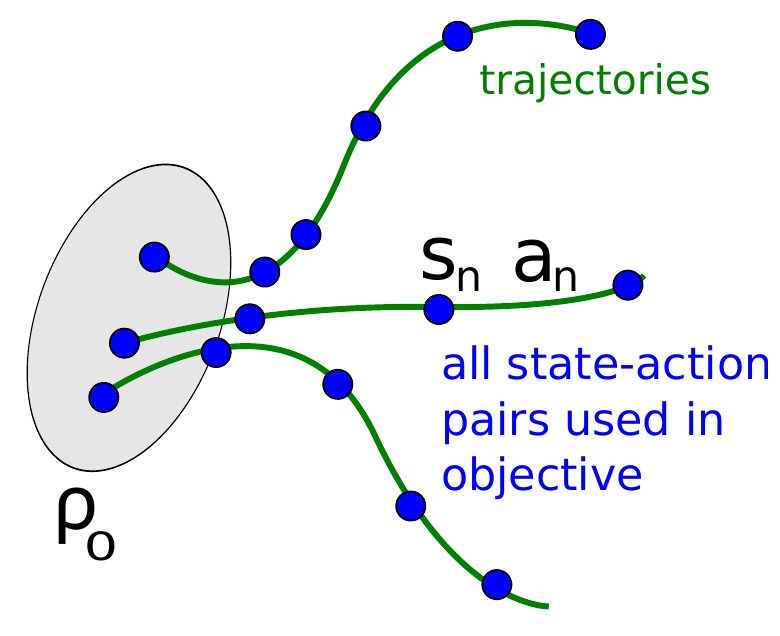
\includegraphics[height=3.2cm]{trpo_single_path.png}\par\raggedright
\begin{itemize}
  \item Roll out $\pi_{\told}$; use \textbf{every} $(s_n,a_n)$.
  \item $q=\pi_{\told}$; $\hat Q$ = discounted return-to-go.
  \item \textbf{No state resets} --- works on real systems.
\end{itemize}
\end{warmbox}
\begin{coolbox}[title={Vine}]
\centering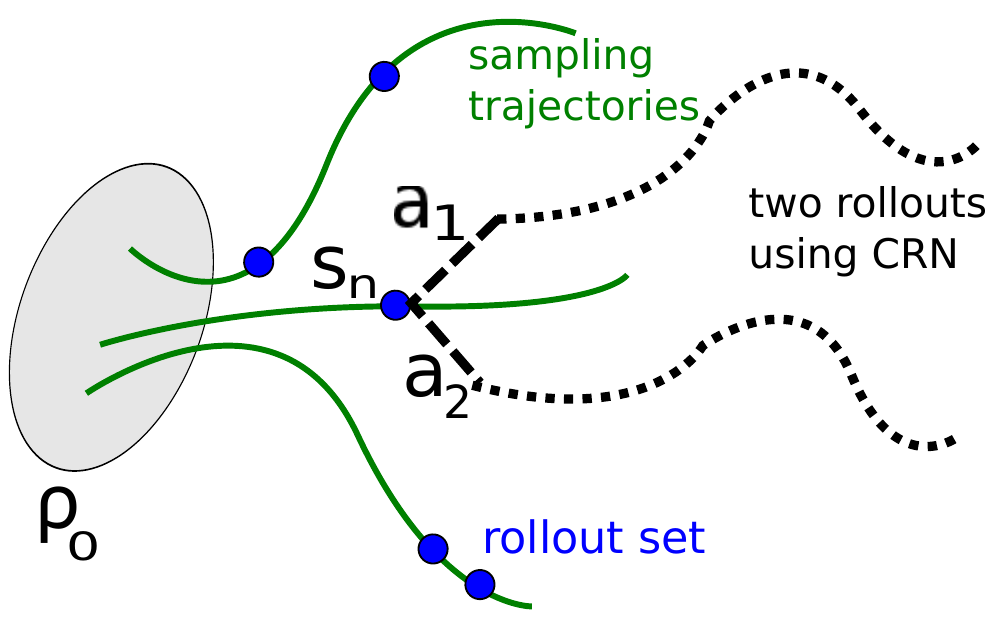
\includegraphics[height=3.2cm]{trpo_vine.png}\par\raggedright
\begin{itemize}
  \item From each $s_n$ in a \textbf{rollout set}: try $K$ actions $a_k\sim q$, a short rollout each, with common random numbers.
  \item \textbf{Lower-variance} $\hat Q$.
  \item Needs \textbf{resets} --- but only to states reached from $\rho_0$: \textbf{not} CPI's $\mu$.
\end{itemize}
\end{coolbox}
\end{pair}

{\small $q=\pi_{\theta_i}$ for continuous control, uniform for Atari (``can sometimes achieve better exploration'' --- over actions, at states already visited). Vine with continuous actions uses self-normalized IS, which removes the need for a baseline. Figures: TRPO Fig.~1.}

\subsection{4. Linear objective, quadratic constraint: the search direction}
\trpostep{4}

Approximate around $\told$:
\begin{gather*}
  L(\theta) \approx L(\told) + g^\top(\theta - \told), \qquad
  \bar D_{\mathrm{KL}}(\told,\theta) \approx \tfrac12(\theta-\told)^\top A\,(\theta-\told)
\end{gather*}

\begin{enumerate}
  \item $A_{ij}=\frac{\partial^2}{\partial\theta_i\partial\theta_j}\bar D_{\mathrm{KL}}(\told,\theta)$: the \textbf{curvature of the KL} --- the \textbf{Fisher information matrix}. Computed analytically, not from sampled score functions.
  \item The KL has \textbf{no linear term}: it is minimized (zero) at $\theta=\told$, so its gradient vanishes there.
  \item Solution direction $s\propto A^{-1}g$: the \textbf{natural gradient} --- steepest ascent when distance is measured in KL, not in $\|\theta\|$.
\end{enumerate}

\simp{$L$ and the KL are nonlinear in $\theta$; an exact constrained solve per batch is too expensive.}
     {First/second-order Taylor models $\Rightarrow$ a closed-form direction $A^{-1}g$.}
     {Valid only locally --- the step must be checked (next).}

{\small With $A^{-1}g$ and a \emph{fixed} step size we would get Kakade's (2002) natural policy gradient; TRPO enforces the constraint at each step instead (App.~\ref{app:trpo-conn}).}

\subsection{5. Computing the step: conjugate gradient + line search}
\trpostep{5}

\begin{minipage}[c]{0.54\linewidth}
\begin{enumerate}
  \item \textbf{Direction:} solve $A\,s=g$ by \textbf{conjugate gradient}. It needs only products $y\mapsto Ay$ (autodiff), $k=10$ iterations. $A$ has $|\theta|^2$ entries and is never formed.
  \item \textbf{Largest step to the KL boundary} of the quadratic model:
  \begin{gather*}
    \tfrac12(\beta s)^\top A(\beta s)=\delta \;\Rightarrow\; \beta=\sqrt{2\delta/s^\top A s}
  \end{gather*}
  \item \textbf{Backtrack} $\beta,\ \beta/2,\ \beta/4,\dots$ until
  \begin{gather*}
    L_{\told}(\theta)\ \text{improves} \ \ \text{and}\ \ \bar D_{\mathrm{KL}}(\told,\theta)\le\delta.
  \end{gather*}
\end{enumerate}
\end{minipage}\hfill
\begin{minipage}[c]{0.42\linewidth}
\centering
\begin{tikzpicture}[>=Stealth, font=\scriptsize]
  \draw[AtlasCool, thick, rotate=25] (0,0) ellipse (2.1 and 1.0);
  \draw[BadRed, thick, dashed] plot[smooth cycle] coordinates {(-1.6,-0.4)(-0.9,0.5)(0.3,0.8)(1.2,0.6)(0.9,-0.2)(-0.2,-0.7)};
  \fill[AtlasInk] (0,0) circle (1.5pt) node[below left] {$\told$};
  \draw[->, thick, AtlasSlate] (0,0) -- (1.85,0.85) node[right] {$\beta s$};
  \draw[->, thick, AtlasSlate!70] (0,0) -- (0.93,0.43) node[above] {$\beta/2$};
  \fill[GoodGreen] (0.46,0.21) circle (2pt);
  \node[GoodGreen!60!black] at (0.75,-0.05) {$\beta/4$ \cmark};
  \node[AtlasCool] at (0.6,1.55) {quadratic model of KL $=\delta$};
  \node[BadRed] at (-0.6,-1.05) {true $\bar D_{\mathrm{KL}}\le\delta$};
\end{tikzpicture}\\
{\scriptsize Illustrative: the full step and $\beta/2$ fail the true checks, $\beta/4$ passes.}
\end{minipage}

\simp{$A$ cannot even be stored for a neural net; the quadratic model is only local.}
     {CG with Fisher-vector products; a full step to $\delta$; a line search on the true $L$ and KL.}
     {Second order and \textbf{one step per batch} --- PPO's starting point.}

\begin{notebox}
\textbf{Fisher-vector products.} If the network outputs distribution parameters $\mu_\theta(x)$, then $A=J^\top MJ$ with $J=\partial\mu/\partial\theta$ and $M$ the analytic Fisher matrix of the distribution w.r.t.\ $\mu$. $Jy$ and $J^\top v$ are a forward-mode and a backprop pass. FVPs on $\sim$10\% of the data, so one update costs about one gradient. Without the line search, the paper reports occasional large steps with catastrophic drops.
\end{notebox}

% ---------------------------------------------------------------------------
\section{The TRPO algorithm}
% ---------------------------------------------------------------------------

\begin{algbox}{TRPO (one iteration)}
\begin{enumerate}
  \item Collect $(s,a)$ pairs with Monte Carlo $\hat Q$ estimates (single path or vine).
  \item Build the sample estimates of the surrogate $L$ and the mean-KL constraint.
  \item Compute $g=\nabla_\theta L$; solve $As=g$ with conjugate gradient (Fisher-vector products).
  \item Step size $\beta=\sqrt{2\delta/s^\top As}$; backtracking line search on $L$ and the KL.
  \item $\told\leftarrow\told+\beta s$.
\end{enumerate}
Cost per update: only slightly more than computing the gradient itself.
\end{algbox}

\subsection{Recap: from theory to practice}

\begin{center}
\begin{tikzpicture}[>=Stealth, node distance=0.35cm,
    box/.style={fl, cbox=AtlasCool, font=\scriptsize, minimum height=0.95cm, text width=2.6cm}]
  \node[box] (a) {CPI bound\\(mixtures, $\alpha$)};
  \node[box, right=of a] (b) {Thm.~1\\($\DTV^{\max}$)};
  \node[box, right=of b] (c) {KL penalty\\(MM, monotone)};
  \node[box, right=of c, cbox=AtlasSlate] (d) {Trust region\\($\DKL^{\max}\le\delta$)};
  \node[box, below=0.9cm of d, cbox=AtlasSlate] (e) {Mean KL\\($\bar D_{\mathrm{KL}}\le\delta$)};
  \node[box, left=of e, cbox=AtlasSlate] (f) {Samples + IS\\(single path / vine)};
  \node[box, left=of f, cbox=AtlasSlate] (g) {Linear + quadratic\\(natural gradient)};
  \node[box, left=of g, cbox=AtlasWarm] (h) {CG + line search\\(\textbf{TRPO})};
  \foreach \x/\y in {a/b, b/c, c/d, d/e, e/f, f/g, g/h} \draw[->, thick, AtlasSlate] (\x) -- (\y);
  \draw[decorate, decoration={brace, amplitude=5pt}, GoodGreen, thick] ([yshift=4pt]a.north west) -- node[above=6pt, font=\scriptsize]{theory: monotone improvement} ([yshift=4pt]c.north east);
\end{tikzpicture}
\end{center}

\begin{itemize}
  \item First three boxes: \textbf{theory}. From the trust region on: \textbf{practice} --- each arrow trades a guarantee for practicality.
  \item The theory ignores advantage-estimation error (K\&L handle it; TRPO omits it for simplicity).
  \item What is left: noisy $\hat Q$ (\textbf{GAE}) and a heavy second-order solver (\textbf{PPO}).
\end{itemize}

% ---------------------------------------------------------------------------
\section{What TRPO does not fix: where the data come from}
\label{sec:trpo-noexplore}
% ---------------------------------------------------------------------------

\begin{center}
\begin{tikzpicture}
\begin{axis}[notes, width=11cm, height=4.2cm, ybar, bar width=6pt, ymin=0, ymax=0.45,
    xtick={1,...,10}, xticklabels={$s_0$,2,3,4,5,6,7,8,9,goal}, ytick=\empty,
    legend style={at={(0.5,1.02)}, anchor=south, legend columns=2}, area legend]
  \addplot[fill=AtlasCool!70, draw=none] coordinates {(1,0.4)(2,0.28)(3,0.17)(4,0.09)(5,0.04)(6,0.015)(7,0.005)(8,0)(9,0)(10,0)};
  \addlegendentry{data: $s\sim\rho_{\piold}$ (from $\rho_0$)}
  \addplot[fill=AtlasAccent!20, draw=AtlasAccent] coordinates {(1,0.06)(2,0.06)(3,0.06)(4,0.06)(5,0.06)(6,0.06)(7,0.06)(8,0.07)(9,0.08)(10,0.37)};
  \addlegendentry{a better policy}
  \draw[GoodGreen, thick, |-|] (axis cs:0.7,0.43) -- node[above, font=\scriptsize]{trust region acts here} (axis cs:6.3,0.43);
  \node[font=\scriptsize, BadRed, align=center] at (axis cs:8.6,0.25) {no samples:\\no weight can fix this};
\end{axis}
\end{tikzpicture}
\end{center}

\begin{enumerate}
  \item \textbf{Data:} $s_0\sim\rho_0$, then $\piold$ --- CPI's $\mu$ is gone.
  \item \textbf{Trust region:} limits how much $\pi$ changes \textbf{on the states we have}.
  \item \textbf{Importance sampling:} reweights \textbf{actions}, never states.
  \item \textbf{Vine:} resets only to states already reached from $\rho_0$.
\end{enumerate}

\begin{warnbox}[title={Trust region $\neq$ exploration}]
Lane B (CPI's Gap 2, \S\ref{sec:gap2-ex1}) stays open in TRPO, GAE and PPO. The only exploration left is in the actions: a stochastic policy, a uniform $q$ for the vine on Atari, and later PPO's entropy bonus.
\end{warnbox}

{\small Why TRPO still works in the experiments: $\rho_0$ and a stochastic policy already cover the relevant states (locomotion from a standing pose, Atari from the start screen).}

% ---------------------------------------------------------------------------
\section{Results}
\label{sec:trpo-results}
% ---------------------------------------------------------------------------

\subsection{Simulated robots (MuJoCo)}

\begin{minipage}[c]{0.52\linewidth}
\centering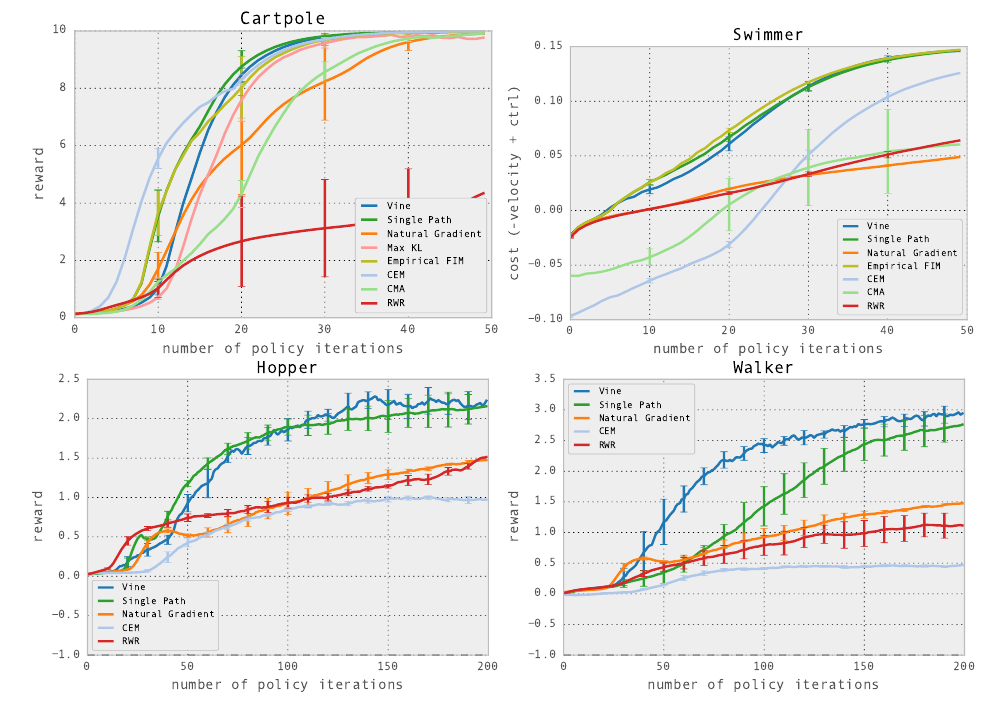
\includegraphics[width=\linewidth]{trpo_fig4_mujoco.png}\\
{\scriptsize TRPO Fig.~4: learning curves, five runs.}
\end{minipage}\hfill
\begin{minipage}[c]{0.45\linewidth}
\begin{itemize}
  \item Swimmer, hopper, walker: torques from joint states; neural-net policies.
  \item {\color{AtlasCool}\textbf{Vine, single path}}: solve all tasks, best scores.
  \item \textbf{Natural gradient} (fixed step): no hopping or walking gait.
  \item \textbf{CEM, CMA} (derivative-free): poor on the larger networks.
  \item \textbf{Max KL} (cart-pole only): a bit slower than mean KL --- simplification 2 costs little.
  \item Same $\delta=0.01$ in every experiment.
\end{itemize}
\end{minipage}

\subsection{Atari from raw pixels}

\begin{center}
\footnotesize
\setlength{\tabcolsep}{5pt}
\begin{tabular}{l r r r r r r r}
\toprule
 & B.\,Rider & Breakout & Enduro & Pong & Q*bert & Seaquest & S.\,Invaders \\
\midrule
{\color{NoteGray}Random} & {\color{NoteGray}354} & {\color{NoteGray}1.2} & {\color{NoteGray}0} & {\color{NoteGray}$-20.4$} & {\color{NoteGray}157} & {\color{NoteGray}110} & {\color{NoteGray}179} \\
{\color{NoteGray}Human} & {\color{NoteGray}7456} & {\color{NoteGray}31.0} & {\color{NoteGray}368} & {\color{NoteGray}$-3.0$} & {\color{NoteGray}18900} & {\color{NoteGray}28010} & {\color{NoteGray}3690} \\
Deep Q-learning & 4092 & 168.0 & 470 & 20.0 & 1952 & 1705 & 581 \\
UCC-I (MCTS) & 5702 & 380 & 741 & 21 & 20025 & 2995 & 692 \\
\midrule
{\color{AtlasCool}\textbf{TRPO single path}} & 1425.2 & 10.8 & \textbf{534.6} & \textbf{20.9} & \textbf{1973.5} & \textbf{1908.6} & 568.4 \\
{\color{AtlasCool}\textbf{TRPO vine}} & 859.5 & 34.2 & 430.8 & \textbf{20.9} & \textbf{7732.5} & 788.4 & 450.2 \\
\bottomrule
\end{tabular}\\[2pt]
{\scriptsize\color{NoteGray}TRPO Table~1. Bold: TRPO above Deep Q-learning. One run per game.}
\end{center}

\begin{keybox}
Not built for games --- yet the \textbf{same} algorithm and settings as for the robots give reasonable scores everywhere. (CNN policy with 33{,}500 parameters; 500 iterations $\approx$ 30 hours on 16 cores.)
\end{keybox}
